\chapter{Cap\'itulo 1}
\label{ch:cap1}

\lipsum[1]

O Instituto Nacional de Pesquisas Espaciais (INPE) desenvolve sat\'elites para o monitoramento da Terra. Exemplos desat\'elites desenvolvidos pelo INPE s\~ao o Data Collection Satellite (SCD-1 and SCD-2, ver Figura~\ref{fig:scd}), o China-Brazil Earth Resources Satellite Program (CBERS-1, CBERS-2, CBERS-2B, CBERS-3, CBERS-4, ver Figura~\ref{fig:cbers}) e o Amaz\^onia project (Amaz\^onia-1, ver Figura~\ref{fig:amazonia}).

\begin{figure}[!htb]
    \centering
    \begin{minipage}{0.5\textwidth}
        \centering
        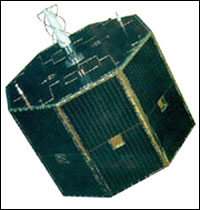
\includegraphics[trim=5 5 5 5, clip, width=0.4\linewidth]{./figuras/scd1_2}
        \caption{SCD-1}
        \label{fig:scd}
    \end{minipage}%
    \begin{minipage}{0.5\textwidth}
        \centering
        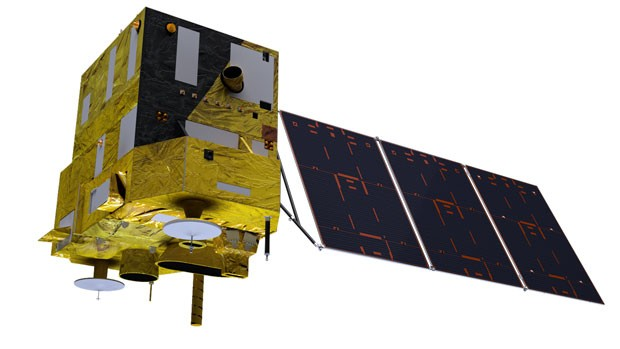
\includegraphics[width=0.7\linewidth]{./figuras/Cbers1}
        \caption{CBERS-3}
        \label{fig:cbers}
    \end{minipage}
    
    \vspace{1em}
    
    \begin{minipage}{0.5\textwidth}
        \centering
        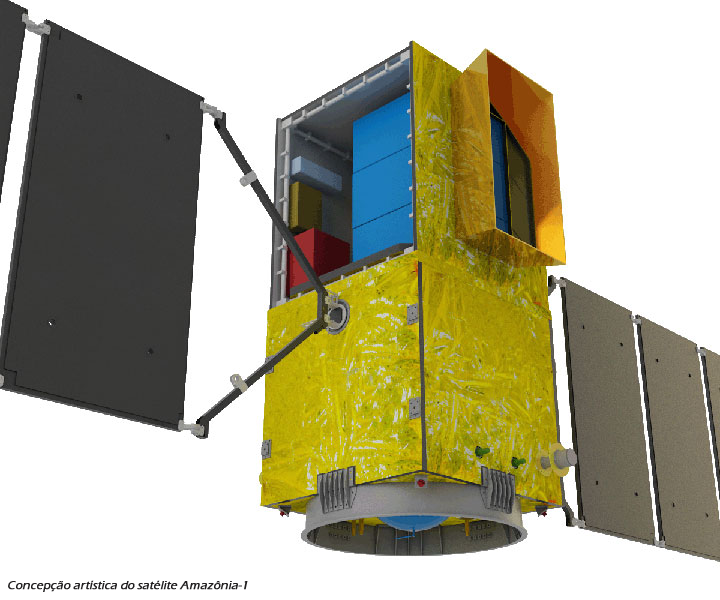
\includegraphics[width=0.7\linewidth]{./figuras/Amazonia-1}
        \caption{Amaz\^onia-1}
        \label{fig:amazonia}
    \end{minipage}
\end{figure}